\documentclass[12pt]{article}
\usepackage{fancyhdr}
\usepackage{color}
\usepackage{multicol}
\usepackage{enumitem}
\usepackage{graphicx}
\usepackage{sectsty}
\usepackage{amsmath}
\usepackage{amssymb}
\usepackage{hyperref}
\usepackage{array}
\newcommand{\sectionbreak}{\clearpage}

\allsectionsfont{\centering}

\usepackage{draftwatermark}
	\SetWatermarkText{\copyright wolf-math.com}
	\SetWatermarkScale{4}
	\SetWatermarkLightness{1}

\usepackage[margin=1in, headsep=0pt]{geometry}
\setlength{\parindent}{0cm}
\pagestyle{empty}

\begin{document}

Mr. Wolf  \\ CMSD-JFK\\2014-2015

\section*{Triangles: Congruence, Similarity \& Trig Ratios}

\subsection*{Goals \& Objectives}

\textbf{I will be able to} calculate the measure of unknown angles in a triangle by using \textit{The Triangle Angle-Sum Theorem}.\\

\textbf{I will be able to} set up a trigonometric ratio in a right triangle.\\

\textbf{I will be able to} use trig ratios to solve for unknown sides of a right triangle.\\

\subsection*{Standards}

\textbf{Congruence \hfill G-CO}\\

Understand congruence and similarity using physical models, transparencies, or geometry software.\\

\begin{enumerate}

	\item[5.] Use informal arguments to establish facts about the angle sum and exterior angle of triangles, about the angles created when parallel lines are cut by a transversal, and the angle-angle criterion for similarity of triangles. For example, arrange three copies of the same triangle so that the sum of the three angles appears to form a line, and give an argument in terms of transversals why this is so.

\end{enumerate}



\textbf{Similarity, Right Triangles, and Trigonometry \hfill G-SRT}\\

Understand similarity in terms of similarity transformations\\

\begin{enumerate}


\item Verify experimentally the properties of dilations given by a center and
	a scale factor:

	\begin{enumerate}
		\item A dilation takes a line not passing through the center of the dilation to a parallel line, and leaves a line passing through the center unchanged.\\
		
		\item The dilation of a line segment is longer or shorter in the ratio given by the scale factor.\\
	\end{enumerate}

\item Given two figures, use the definition of similarity in terms of similarity transformations to decide if they are similar; explain using similarity transformations the meaning of similarity for triangles as the equality of all corresponding pairs of angles and the proportionality of all corresponding pairs of sides.\\

\item Use the properties of similarity transformations to establish the AA criterion for two triangles to be similar. Prove theorems involving similarity\\

\item 4. Prove theorems about triangles. Theorems include: a line parallel to one side of a triangle divides the other two proportionally, and conversely; the Pythagorean Theorem proved using triangle similarity.\\

\item  Use congruence and similarity criteria for triangles to solve problems and to prove relationships in geometric figures. Define trigonometric ratios and solve problems involving right triangles\\

\item  Understand that by similarity, side ratios in right triangles are
properties of the angles in the triangle, leading to definitions of trigonometric ratios for acute angles.\\

\item  Explain and use the relationship between the sine and cosine of complementary angles.\\

\item  Use trigonometric ratios and the Pythagorean Theorem to solve right triangles in applied problems.\\

\end{enumerate}

\subsection*{Connections}

\textbf{Before:} We learned simplifying radicals, the Pythaorean Theorem, the Distance Formula, and the equation of a circle. These were all in preparation for trigonometry.\\

\textbf{After:} We will put the trigonometry we learned onto the coordinate plane and apply these concepts in the unit circle and graphing trigonometric functions.\

\let\stdsection\section
\renewcommand\section{\newpage\stdsection}

\section*{Angle Sum Theorem}

The \textbf{sum} of the measures of the interior angles of a triangle is $180^{\circ}$\\

\begin{center}
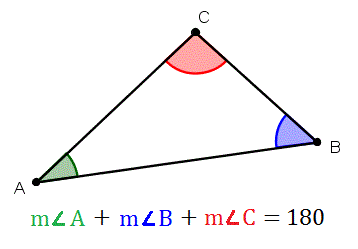
\includegraphics[scale=.5]{triangle2.png}\\
\end{center}

What this means is that as long as two angles are known, the third one can be figured out.\\

What is the measure of angle $C$?\\

\begin{center}
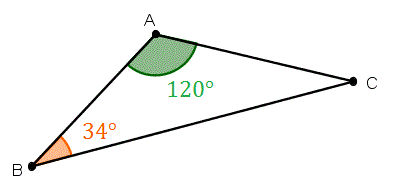
\includegraphics[scale=.5]{triangle3.png}
\end{center}

\hrulefill

\textbf{You Try:} Find the measure of angle $B$.\\

\begin{center}
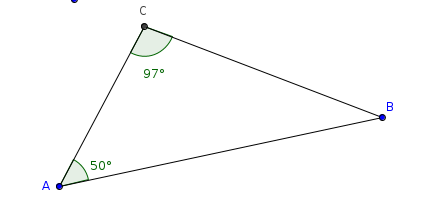
\includegraphics[scale=.5]{triangle4.png}\\
\end{center}

Find the measure of $x$.\\

\begin{center}
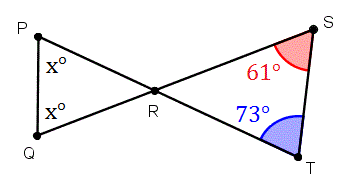
\includegraphics[scale=.5]{triangle5.png}
\end{center}

\subsection*{Exterior Angles of a Triangle}

An \textbf{Exterior Angle} is when one side of a triangle is extended, and an additional angle is created \textit{outside} of the triangle.\\

\begin{center}
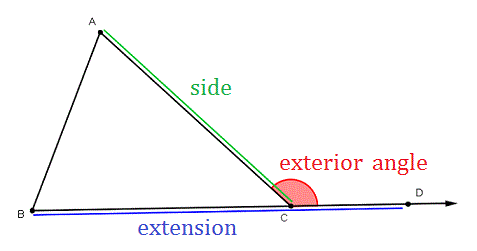
\includegraphics[scale=.6]{triangle6.png}\\
\end{center}

The angles that are opposite of the exterior angle are called \textbf{Remote Interior Angles}.

\begin{center}
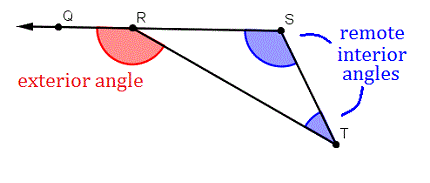
\includegraphics[scale=.5]{triangle7.png}
\end{center}

\subsection*{Exterior Angle Theorem}

The \textbf{Exterior Angle Theorem} states that the measure of an exterior angle is equal to the sum of the measures of the remote interior angles.\\

\begin{center}
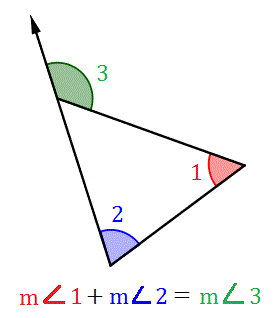
\includegraphics[scale=.6]{triangle8.png}\\
\end{center}

Try to find $m\angle 1$ and $m\angle 2$\\

\begin{center}
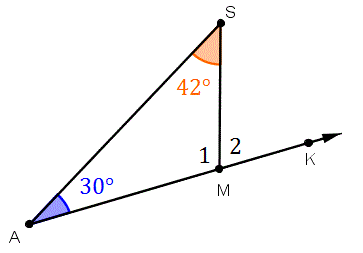
\includegraphics[scale=.5]{triangle9.png}
\end{center}


\section*{Congruence \& Similarity}

\textbf{Congruence} is another way of saying same size and shape.\\

\textbf{Similarity} is another way of saying same size, but different shape.\\

\textbf{Example:} If you go to a car dealership and find two brand new Porches, they are congruent to one another. However, if you compare one brand new Porche to my desktop scale model, then it's similar. The first two are exactly the same size and shape, and the the second two are the same shape, but different sizes.\\

\hrulefill

\subsection*{Hypotenuse Leg (HL) Theorem}

The \textbf{Hypotenuse Leg Theorem} states that if the hypotenuse and one (1) leg of a triangle are congruent, then the two triangles are congruent. \\

\begin{center}
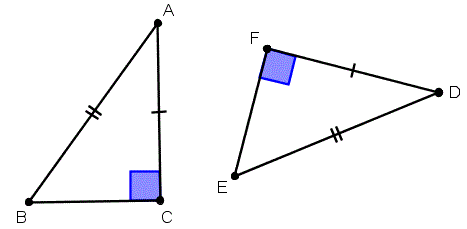
\includegraphics[scale=.5]{triangle10.png}
\end{center}

The two right triangles above have congruent hypotenuses and one congruent leg. That means that they are congruent, and the unmarked legs are also congruent.\\

\hrulefill

What additional information is needed in order to determine if the triangles below are congruent?\\

\begin{center}
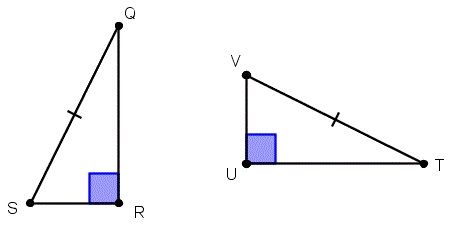
\includegraphics[scale=.5]{triangle12.png}
\end{center}



\end{document}